
%% bare_conf.tex
%% V1.3
%% 2007/01/11
%% by Michael Shell
%% See:
%% http://www.michaelshell.org/
%% for current contact information.
%%
%% This is a skeleton file demonstrating the use of IEEEtran.cls
%% (requires IEEEtran.cls version 1.7 or later) with an IEEE conference paper.
%%
%% Support sites:
%% http://www.michaelshell.org/tex/ieeetran/
%% http://www.ctan.org/tex-archive/macros/latex/contrib/IEEEtran/
%% and
%% http://www.ieee.org/

%%*************************************************************************
%% Legal Notice:
%% This code is offered as-is without any warranty either expressed or
%% implied; without even the implied warranty of MERCHANTABILITY or
%% FITNESS FOR A PARTICULAR PURPOSE! 
%% User assumes all risk.
%% In no event shall IEEE or any contributor to this code be liable for
%% any damages or losses, including, but not limited to, incidental,
%% consequential, or any other damages, resulting from the use or misuse
%% of any information contained here.
%%
%% All comments are the opinions of their respective authors and are not
%% necessarily endorsed by the IEEE.
%%
%% This work is distributed under the LaTeX Project Public License (LPPL)
%% ( http://www.latex-project.org/ ) version 1.3, and may be freely used,
%% distributed and modified. A copy of the LPPL, version 1.3, is included
%% in the base LaTeX documentation of all distributions of LaTeX released
%% 2003/12/01 or later.
%% Retain all contribution notices and credits.
%% ** Modified files should be clearly indicated as such, including  **
%% ** renaming them and changing author support contact information. **
%%
%% File list of work: IEEEtran.cls, IEEEtran_HOWTO.pdf, bare_adv.tex,
%%                    bare_conf.tex, bare_jrnl.tex, bare_jrnl_compsoc.tex
%%*************************************************************************

% *** Authors should verify (and, if needed, correct) their LaTeX system  ***
% *** with the testflow diagnostic prior to trusting their LaTeX platform ***
% *** with production work. IEEE's font choices can trigger bugs that do  ***
% *** not appear when using other class files.                            ***
% The testflow support page is at:
% http://www.michaelshell.org/tex/testflow/



% Note that the a4paper option is mainly intended so that authors in
% countries using A4 can easily print to A4 and see how their papers will
% look in print - the typesetting of the document will not typically be
% affected with changes in paper size (but the bottom and side margins will).
% Use the testflow package mentioned above to verify correct handling of
% both paper sizes by the user's LaTeX system.
%
% Also note that the "draftcls" or "draftclsnofoot", not "draft", option
% should be used if it is desired that the figures are to be displayed in
% draft mode.
%
\documentclass[conference]{IEEEtran}

\IEEEoverridecommandlockouts
% Add the compsoc option for Computer Society conferences.
%
% If IEEEtran.cls has not been installed into the LaTeX system files,
% manually specify the path to it like:
% \documentclass[conference]{../sty/IEEEtran}





% Some very useful LaTeX packages include:
% (uncomment the ones you want to load)


% *** MISC UTILITY PACKAGES ***
%
%\usepackage{ifpdf}
% Heiko Oberdiek's ifpdf.sty is very useful if you need conditional
% compilation based on whether the output is pdf or dvi.
% usage:
% \ifpdf
%   % pdf code
% \else
%   % dvi code
% \fi
% The latest version of ifpdf.sty can be obtained from:
% http://www.ctan.org/tex-archive/macros/latex/contrib/oberdiek/
% Also, note that IEEEtran.cls V1.7 and later provides a builtin
% \ifCLASSINFOpdf conditional that works the same way.
% When switching from latex to pdflatex and vice-versa, the compiler may
% have to be run twice to clear warning/error messages.






% *** CITATION PACKAGES ***
%
%\usepackage{cite}
% cite.sty was written by Donald Arseneau
% V1.6 and later of IEEEtran pre-defines the format of the cite.sty package
% \cite{} output to follow that of IEEE. Loading the cite package will
% result in citation numbers being automatically sorted and properly
% "compressed/ranged". e.g., [1], [9], [2], [7], [5], [6] without using
% cite.sty will become [1], [2], [5]--[7], [9] using cite.sty. cite.sty's
% \cite will automatically add leading space, if needed. Use cite.sty's
% noadjust option (cite.sty V3.8 and later) if you want to turn this off.
% cite.sty is already installed on most LaTeX systems. Be sure and use
% version 4.0 (2003-05-27) and later if using hyperref.sty. cite.sty does
% not currently provide for hyperlinked citations.
% The latest version can be obtained at:
% http://www.ctan.org/tex-archive/macros/latex/contrib/cite/
% The documentation is contained in the cite.sty file itself.






% *** GRAPHICS RELATED PACKAGES ***
%
\ifCLASSINFOpdf
  \usepackage[pdftex]{graphicx}
  % declare the path(s) where your graphic files are
  \graphicspath{{media}}
  % and their extensions so you won't have to specify these with
  % every instance of \includegraphics
  \DeclareGraphicsExtensions{.pdf,.jpeg,.png}
\else
  % or other class option (dvipsone, dvipdf, if not using dvips). graphicx
  % will default to the driver specified in the system graphics.cfg if no
  % driver is specified.
  % \usepackage[dvips]{graphicx}
  % declare the path(s) where your graphic files are
  % \graphicspath{{../eps/}}
  % and their extensions so you won't have to specify these with
  % every instance of \includegraphics
  % \DeclareGraphicsExtensions{.eps}
\fi
% graphicx was written by David Carlisle and Sebastian Rahtz. It is
% required if you want graphics, photos, etc. graphicx.sty is already
% installed on most LaTeX systems. The latest version and documentation can
% be obtained at: 
% http://www.ctan.org/tex-archive/macros/latex/required/graphics/
% Another good source of documentation is "Using Imported Graphics in
% LaTeX2e" by Keith Reckdahl which can be found as epslatex.ps or
% epslatex.pdf at: http://www.ctan.org/tex-archive/info/
%
% latex, and pdflatex in dvi mode, support graphics in encapsulated
% postscript (.eps) format. pdflatex in pdf mode supports graphics
% in .pdf, .jpeg, .png and .mps (metapost) formats. Users should ensure
% that all non-photo figures use a vector format (.eps, .pdf, .mps) and
% not a bitmapped formats (.jpeg, .png). IEEE frowns on bitmapped formats
% which can result in "jaggedy"/blurry rendering of lines and letters as
% well as large increases in file sizes.
%
% You can find documentation about the pdfTeX application at:
% http://www.tug.org/applications/pdftex





% *** MATH PACKAGES ***
%
\usepackage[cmex10]{amsmath}
% A popular package from the American Mathematical Society that provides
% many useful and powerful commands for dealing with mathematics. If using
% it, be sure to load this package with the cmex10 option to ensure that
% only type 1 fonts will utilized at all point sizes. Without this option,
% it is possible that some math symbols, particularly those within
% footnotes, will be rendered in bitmap form which will result in a
% document that can not be IEEE Xplore compliant!
%
% Also, note that the amsmath package sets \interdisplaylinepenalty to 10000
% thus preventing page breaks from occurring within multiline equations. Use:
%\interdisplaylinepenalty=2500
% after loading amsmath to restore such page breaks as IEEEtran.cls normally
% does. amsmath.sty is already installed on most LaTeX systems. The latest
% version and documentation can be obtained at:
% http://www.ctan.org/tex-archive/macros/latex/required/amslatex/math/





% *** SPECIALIZED LIST PACKAGES ***
%
%\usepackage{algorithmic}
% algorithmic.sty was written by Peter Williams and Rogerio Brito.
% This package provides an algorithmic environment fo describing algorithms.
% You can use the algorithmic environment in-text or within a figure
% environment to provide for a floating algorithm. Do NOT use the algorithm
% floating environment provided by algorithm.sty (by the same authors) or
% algorithm2e.sty (by Christophe Fiorio) as IEEE does not use dedicated
% algorithm float types and packages that provide these will not provide
% correct IEEE style captions. The latest version and documentation of
% algorithmic.sty can be obtained at:
% http://www.ctan.org/tex-archive/macros/latex/contrib/algorithms/
% There is also a support site at:
% http://algorithms.berlios.de/index.html
% Also of interest may be the (relatively newer and more customizable)
% algorithmicx.sty package by Szasz Janos:
% http://www.ctan.org/tex-archive/macros/latex/contrib/algorithmicx/




% *** ALIGNMENT PACKAGES ***
%
%\usepackage{array}
% Frank Mittelbach's and David Carlisle's array.sty patches and improves
% the standard LaTeX2e array and tabular environments to provide better
% appearance and additional user controls. As the default LaTeX2e table
% generation code is lacking to the point of almost being broken with
% respect to the quality of the end results, all users are strongly
% advised to use an enhanced (at the very least that provided by array.sty)
% set of table tools. array.sty is already installed on most systems. The
% latest version and documentation can be obtained at:
% http://www.ctan.org/tex-archive/macros/latex/required/tools/


%\usepackage{mdwmath}
%\usepackage{mdwtab}
% Also highly recommended is Mark Wooding's extremely powerful MDW tools,
% especially mdwmath.sty and mdwtab.sty which are used to format equations
% and tables, respectively. The MDWtools set is already installed on most
% LaTeX systems. The lastest version and documentation is available at:
% http://www.ctan.org/tex-archive/macros/latex/contrib/mdwtools/


% IEEEtran contains the IEEEeqnarray family of commands that can be used to
% generate multiline equations as well as matrices, tables, etc., of high
% quality.


%\usepackage{eqparbox}
% Also of notable interest is Scott Pakin's eqparbox package for creating
% (automatically sized) equal width boxes - aka "natural width parboxes".
% Available at:
% http://www.ctan.org/tex-archive/macros/latex/contrib/eqparbox/





% *** SUBFIGURE PACKAGES ***
%\usepackage[tight,footnotesize]{subfigure}
% subfigure.sty was written by Steven Douglas Cochran. This package makes it
% easy to put subfigures in your figures. e.g., "Figure 1a and 1b". For IEEE
% work, it is a good idea to load it with the tight package option to reduce
% the amount of white space around the subfigures. subfigure.sty is already
% installed on most LaTeX systems. The latest version and documentation can
% be obtained at:
% http://www.ctan.org/tex-archive/obsolete/macros/latex/contrib/subfigure/
% subfigure.sty has been superceeded by subfig.sty.



%\usepackage[caption=false]{caption}
%\usepackage[font=footnotesize]{subfig}
% subfig.sty, also written by Steven Douglas Cochran, is the modern
% replacement for subfigure.sty. However, subfig.sty requires and
% automatically loads Axel Sommerfeldt's caption.sty which will override
% IEEEtran.cls handling of captions and this will result in nonIEEE style
% figure/table captions. To prevent this problem, be sure and preload
% caption.sty with its "caption=false" package option. This is will preserve
% IEEEtran.cls handing of captions. Version 1.3 (2005/06/28) and later 
% (recommended due to many improvements over 1.2) of subfig.sty supports
% the caption=false option directly:
%\usepackage[caption=false,font=footnotesize]{subfig}
%
% The latest version and documentation can be obtained at:
% http://www.ctan.org/tex-archive/macros/latex/contrib/subfig/
% The latest version and documentation of caption.sty can be obtained at:
% http://www.ctan.org/tex-archive/macros/latex/contrib/caption/




% *** FLOAT PACKAGES ***
%
%\usepackage{fixltx2e}
% fixltx2e, the successor to the earlier fix2col.sty, was written by
% Frank Mittelbach and David Carlisle. This package corrects a few problems
% in the LaTeX2e kernel, the most notable of which is that in current
% LaTeX2e releases, the ordering of single and double column floats is not
% guaranteed to be preserved. Thus, an unpatched LaTeX2e can allow a
% single column figure to be placed prior to an earlier double column
% figure. The latest version and documentation can be found at:
% http://www.ctan.org/tex-archive/macros/latex/base/



%\usepackage{stfloats}
% stfloats.sty was written by Sigitas Tolusis. This package gives LaTeX2e
% the ability to do double column floats at the bottom of the page as well
% as the top. (e.g., "\begin{figure*}[!b]" is not normally possible in
% LaTeX2e). It also provides a command:
%\fnbelowfloat
% to enable the placement of footnotes below bottom floats (the standard
% LaTeX2e kernel puts them above bottom floats). This is an invasive package
% which rewrites many portions of the LaTeX2e float routines. It may not work
% with other packages that modify the LaTeX2e float routines. The latest
% version and documentation can be obtained at:
% http://www.ctan.org/tex-archive/macros/latex/contrib/sttools/
% Documentation is contained in the stfloats.sty comments as well as in the
% presfull.pdf file. Do not use the stfloats baselinefloat ability as IEEE
% does not allow \baselineskip to stretch. Authors submitting work to the
% IEEE should note that IEEE rarely uses double column equations and
% that authors should try to avoid such use. Do not be tempted to use the
% cuted.sty or midfloat.sty packages (also by Sigitas Tolusis) as IEEE does
% not format its papers in such ways.





% *** PDF, URL AND HYPERLINK PACKAGES ***
%
\usepackage{url}
% url.sty was written by Donald Arseneau. It provides better support for
% handling and breaking URLs. url.sty is already installed on most LaTeX
% systems. The latest version can be obtained at:
% http://www.ctan.org/tex-archive/macros/latex/contrib/misc/
% Read the url.sty source comments for usage information. Basically,
% \url{my_url_here}.


\usepackage[utf8]{inputenc}


% *** Do not adjust lengths that control margins, column widths, etc. ***
% *** Do not use packages that alter fonts (such as pslatex).         ***
% There should be no need to do such things with IEEEtran.cls V1.6 and later.
% (Unless specifically asked to do so by the journal or conference you plan
% to submit to, of course. )


% correct bad hyphenation here
\hyphenation{op-tical net-works semi-conduc-tor}

% include page numbers
\pagenumbering{arabic}


\begin{document}
%
% paper title
% can use linebreaks \\ within to get better formatting as desired
\title{Survey on Performance Models of Container Networks}


% author names and affiliations
% use a multiple column layout for up to three different
% affiliations
\author{\IEEEauthorblockN{David de Andrés Hernández}
\IEEEauthorblockA{Department of Electrical and Computer Engineering\\
Technical University of Munich\\
Email: deandres.hernandez@tum.de}
%\and
%\IEEEauthorblockN{Your supervisor is NOT! an author of your paper!}
%\IEEEauthorblockA{Starfleet Academy\\
%San Francisco, California 96678-2391\\
%Telephone: (800) 555--1212\\
%Fax: (888) 555--1212}

%\thanks{*This paper is a reinterpretation of the paper \emph{J. Caesar. ``Digital sundials and broadband technology,'' in Proc.
%IOOC-ECOC, 19XX, pp. 557-998}. It was presented on December 24, 2006 (Paper submission deadline) as a part of MSCE Seminar (MSCE course TUM), under the supervision of M. Sc. (or Dipl. Ing.) 
%Aurelia Cotta (aurelia.cotta@roma.it).}
}

% conference papers do not typically use \thanks and this command
% is locked out in conference mode. If really needed, such as for
% the acknowledgment of grants, issue a \IEEEoverridecommandlockouts
% after \documentclass

% for over three affiliations, or if they all won't fit within the width
% of the page, use this alternative format:
% 
%\author{\IEEEauthorblockN{Michael Shell\IEEEauthorrefmark{1},
%Homer Simpson\IEEEauthorrefmark{2},
%James Kirk\IEEEauthorrefmark{3}, 
%Montgomery Scott\IEEEauthorrefmark{3} and
%Eldon Tyrell\IEEEauthorrefmark{4}}
%\IEEEauthorblockA{\IEEEauthorrefmark{1}School of Electrical and Computer Engineering\\
%Georgia Institute of Technology,
%Atlanta, Georgia 30332--0250\\ Email: see http://www.michaelshell.org/contact.html}
%\IEEEauthorblockA{\IEEEauthorrefmark{2}Twentieth Century Fox, Springfield, USA\\
%Email: homer@thesimpsons.com}
%\IEEEauthorblockA{\IEEEauthorrefmark{3}Starfleet Academy, San Francisco, California 96678-2391\\
%Telephone: (800) 555--1212, Fax: (888) 555--1212}
%\IEEEauthorblockA{\IEEEauthorrefmark{4}Tyrell Inc., 123 Replicant Street, Los Angeles, California 90210--4321}}




% use for special paper notices
%\IEEEspecialpapernotice{(Invited Paper)}




% make the title area
\maketitle


\begin{abstract}
%\boldmath
Reliability, scalability, and flexibility are some of the benefits of cloud architectures.  When \textit{cloudifying} any system, the choice of an appropriate container network solution is critical. The wrong container network choice can turn a working system unviable. %This translates into performance degradation, security exposures or unmanageable complexity.
Yet the number of solutions targeting the cloud environment is vast and the angles approaching the challenges are varied. Therefore, understanding and evaluating the benefits and bottlenecks of the available solutions and technologies is a tedious but crucial process. To be thorough, this evaluation requires of several steps. A mandatory first step is to identify the requirements of the system to be \textit{cloudified}. Further, consulting benchmarks and models can give an indication of viability. In the last stages, a high-fidelity model can precisely simulate the results that different configurations and changes can have in the system's behaviour.\\
This paper gives an overview of different container solutions, performance benchmarks and performance models. Finally, the major factors influencing container networks are conceptually introduced.
% Missing closing statement

\end{abstract}

\IEEEpeerreviewmaketitle



\section{Introduction}
% no \IEEEPARstart
Cloud architectures are motivated by both economies of scale and resources optimization and are enabled by virtualization technologies. The cloud promises elasticity, scalability, reliability, availability, and increased operability. However, performance degradation and reduced portability are often the price of virtualization. To mitigate this effect, containers, a form of lightweight virtualization, emerged. Thanks to their alternative means of partitioning resources, the virtualization overhead is drastically reduced, and the deployment process is expedited. These benefits favoured the standardization of containers and that in turn made portability an additional strength of this technology.

Microservices architecture exploits containers even further. This architecture borrows the encapsulation principle of software development and breaks applications into stand-alone containers. In this approach, each container is only responsible for a single function. This function decoupling means that components can be updated or replaced without affecting the remaining components. Moreover, applications can be granularly scaled by load-balancing a function into several instances of the same container. If we take a step further and make individual container instances stateless, containers can be re-spawned, if necessary, without impacting the supported application. The price to pay for microservices is the need of automation and orchestration software to overcome the explosion in the number of components. Overall, microservices and cloud principles are aligned.

We can derive that network connectivity among containers is paramount for their correct functioning.  However, it is not free of challenges. A microservice-populated cloud changes constantly within seconds and containers can be considered ubiquitous. All possible traffic patterns take place: between containers in the same VM, between containers in different VMs, between containers in different hosts, between containers in different data centres, and many more. In this scenario, the host's OS becomes an important element of the networking infrastructure of the cloud. With one remark, it was not conceived for such scale. For this reason, the networking performance of containers must be carefully considered as it can turn a working system unviable when migrated to cloud architectures. The main cause of this degradation is due to overhead processing of packets through the OS's networking stack. Another important factor is that caused by the processing of the headers of overlay networks. To enable the communication of containers in constant move, complex overlay networks are required. But again, the host's OS where not conceived to process efficiently headers at this scale. To overcome the performance challenge, operators have conceived sophisticated frameworks for high-performance packet IO. These frameworks are orthogonal to the network choice but can be leveraged to compensate some of the drawbacks of the selected network.

Cloud networks must also remain extremely flexible as they must often support multi-tenancy while remaining secure. Therefore, flexibility and security are to be considered in the analysis. Due to the immense number of choices for container networking solutions, evaluating the application needs as well as the benefits and bottlenecks of the available solutions is of vital importance.

This survey gives an overview of different solutions for container networking and their underlying technologies. In addition, it presents a collection of available performance benchmarks and models as well as the environments studied so far.  Finally, the major factors influencing container networks are conceptually introduced. 

\section{Background}

\subsection{Networking stacks}
Most container environments make use of the kernel's network stack because it is feature rich, reliable and easy to use. However in high performance scenarios, custom-made stacks running in userspace can replace the kernel's implementation to provide additional performance at the cost of additional complexity.  
\subsubsection{Kernel's stack}

\begin{figure}[!t]
\centering
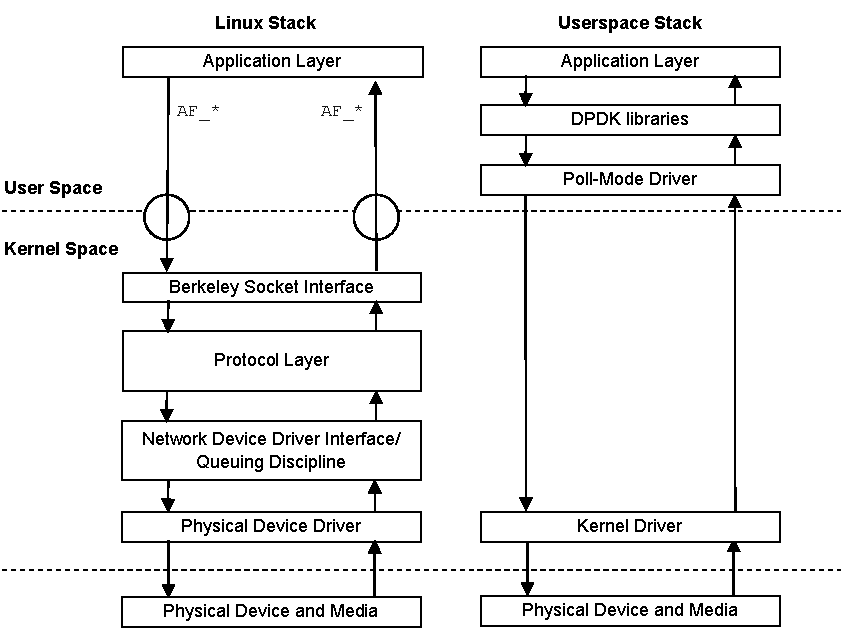
\includegraphics[scale=0.6]{kernel_stack.pdf}
%\includegraphics[width=2.5in]{ }
% where an .eps filename suffix will be assumed under latex, 
% and a .pdf suffix will be assumed for pdflatex; or what has been declared
% via \DeclareGraphicsExtensions.
\caption{Kernel's network stack \cite{kernel_stack} and DPDK stack.}
\label{kernel_stack}
\end{figure}

Current OS's include a rich network stack providing a socket-based user-level interface for transmitting and receiving packets; handling a wide variety of protocols; as well as managing the underlying hardware. Figure \ref{kernel_stack} presents on the left the different layers through which packets must traverse before being handed over to a user-space application. As most of the packet processing, typically up to L4, is performed in kernel space, this collection of layers is often referred to as 'Kernel Networking Stack'.

At the bottom we find the device driver, which is the layer responsible for interacting directly with the HW. This includes: claiming control of a device, requesting memory ranges and IO ports, setting the DMA mask, and registering functions to send,receive and manipulate packets. In the case of virtual devices such as loopback interfaces, TUN, or veth, the drivers are SW only and do not interact with any HW. Next in the stack, we find the Network Device Driver Interface (NDDI), which enables, multiple and perhaps different, network devices to be used simultaneously. Furthermore, the NDDI includes a packet scheduler implementing queuing disciplines. Moving upwards, the protocol layer is where the different protocols are implemented. Each protocol must interact to the north with the socket interface and to the south with the NDDI. To do this, each protocol associates a protocol family (PF\_*) northbound, and a protocol type southbound. At the top of the kernel stack we find the Berkeley Socket Interface, which allows user space programs to communicate with the remote devices. Is effectively the last abstraction layer which gives programs the impression of communicating directly. At this layer, every socket type is associated with a protocol. For example, the PF\_INET is associated with the TCP/IP protocol.

By introducing all these layers, the stack is very flexible and can accommodate features with reduced effort; however, this flexibility is in part responsible for performance loss.

\subsubsection{Userspace stacks}
Although adding complexity by re-implementing the network stack, high-performance IO frameworks are key-enablers for Containerized Network Functions (CNF) \cite{SIGARCH_2017:Yang}. In some occasions the wide variety of protocols and rich functions which the kernel's networking stack offers are not required. This makes it feasible to re-write the required portions of stack using a high-performance IO framework. DPDK \cite{dpdk} and PF\_RING ZC \cite{pf_ring_zc} can lead to a nine-fold performance increase over the default kernel IO framework \cite{ANCS:Gallenmüller}. Figure \ref{kernel_stack} presents on the right the layers of DPDK networking stack. At the bottom we find the kernel driver, a minimal layer which loads and binds the ports to the poll-mode driver in user space. This is the only component which lies within the kernel space. In the user space we find the poll-mode driver. This is a key component to enable high performance. In contrast to the kernel stack which is interrupt-driven, the DPDK stack is polls the NIC continuously. This in turns, consumes all available CPU cycles and in case no packets are available for processing, the CPU cycles are wasted (busy waiting). At the top we find the DPDK libraries, which provide all the elements needed for high-performance packet processing applications. Please refer to \cite{dpdk} for a detailed view of the libraries.\\
Introducing frameworks such as DPDK in container environments has already been accomplished and is a production ready approach. Examples are: Open vSwitch \cite{ovs-dpdk} and Tungsten Fabric \cite{tungsten-dpdk}. The vRouter from the Tungsten Fabric project, for example, leverages DPDK to efficiently route, encapsulate and decapsulate the packets. We see later in section B the importance and performance impact of these operations.

\subsection{Container Networks}
We have seen the importance of container communication in microservices architectures. To materialize this communication, there are multiple options. We differentiate between modes for intra-host and inter-host communication.  Please note that these modes are not exclusive and usually they co-exist.

\begin{figure*}[!t]
\centering
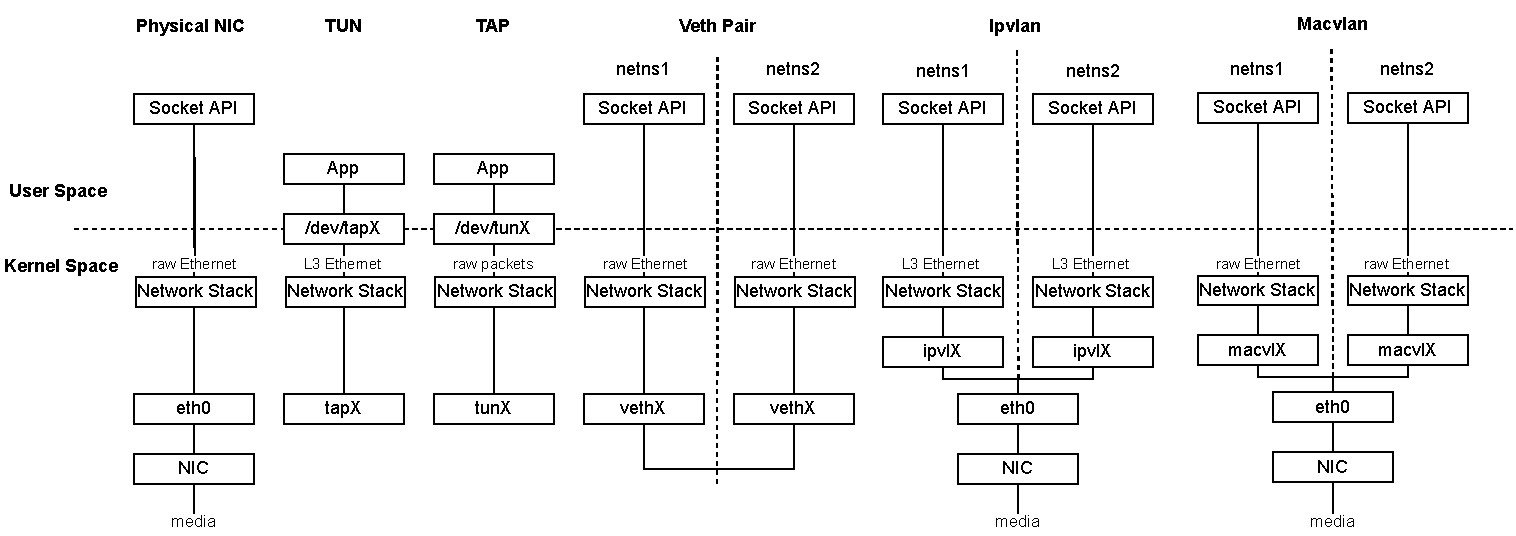
\includegraphics[width=\textwidth]{container_network.drawio.pdf}
%\includegraphics[width=2.5in]{ }
% where an .eps filename suffix will be assumed under latex, 
% and a .pdf suffix will be assumed for pdflatex; or what has been declared
% via \DeclareGraphicsExtensions.
\caption{Available kernel device drivers for container environments}
\label{virtual_networks}
\end{figure*}


\subsubsection{Intra-host communication}\hfill\break
\textbf{None Mode}\hspace{0.2cm}In this mode a container is isolated into its own namespace. This namespace is a logical copy of the OS’s network stack with only a loopback interface. Because of this, it cannot communicate with other containers. Achieving extreme isolation, it is suitable for offline computation such as batch processing or backup jobs.

\noindent\textbf{Bridge Mode}\hspace{0.2cm} In this mode a virtual bridge is created inside a specified namespace. Containers can then be launched including a pair of veth ports, where one of the pairs will be moved to the namespace of the bridge (and enslaved to it) and the other pair will remain in the container's namespace. The veth pair serves as a pipe between both namespaces. Furthermore, the bridge can be enhanced with L3 communication by giving each veth interface an IP address within the bridge's network subnet. This mode allows star-like topologies but does not bring alone connectivity to external networks. For external connectivity other services, such as NAT or overlays must be configured. 

\noindent\textbf{Container Mode}\hspace{0.2cm} The container mode can be seen as an extension of the None mode. First, a container is spawned in None mode, thus creating a dedicated networking namespace. Subsequent containers are launched inside this namespace by providing the namespace's id as a launch parameter. What this effectively does is sharing a single namespace across containers. Therefore, all containers share the access to the interfaces within this namespace as well as firewall rules and ip routes. The level of isolation is reduced but containers benefit from standard inter-process communication (IPC) and hence, suffer less overhead. This mode is often seen in Kubernetes environments under the name of pods. Pods are group of containers belonging to the same user and that work together. In addition, containers can communicate through the loopback interface at the L4 layer.

\noindent\textbf{Host mode} \hspace{0.2cm}In this mode, containers share the host's OS networking stack. Consequently, all containers can communicate with each other through IPC. Additionally, the host can provide external connectivity although sharing the same IP addresses and port ranges. This is the lowest level of security and flexibility. Effectively, host mode can be used as performance baseline as its networking overhead is negligible.

\noindent\textbf{Macvlan}  \hspace{0.2cm} Like VLAN tags, which allow to logically partition a HW interface, Macvlan allows the creation of multiple L2 interfaces with individual MAC addresses on top of a single HW interface. Using Macvlan, a MAC address can be assigned to containers, making it appear as a physical device on the network. To realize this, the Macvlan kernel module enslaves the driver of the NIC in kernel space. The enslaved interfaces now share the same broadcast domain, although whether communication between the interfaces is allowed depends on the configured Macvlan type. There are 5 types, namely: private, VEPA, bridge, passthru and source.\\
Private mode does not allow communication between Macvlan instances, even if the external switch supports hairpin mode. In general, a switch will not return a frame to the same interface it has received it.\\
In VEPA mode, the interface expects a VEPA/802.1Qbg capable switch. The switch acts like a hairpin so frames can be exchanged between the interfaces.\\
In Bridge mode all enslaved interfaces can communicate with each other by means of the physical interface which works as a bridge. In passthru mode, the frames are just passed to the network. So, if a default L2 switch is attached, it works essentially as in private mode.\\
Finally, in source mode, each Macvlan interface receives only frames whose source address has been whitelisted for this interface. This allows the creation of MAC-based VLAN associations.
There is however an important drawback of using Macvlan interfaces: the master interface must be configured in promiscuous mode to allow the forwarding of frames which do not include the master's MAC address. Promiscuous mode in turn needs to be carefully considered in environments with multi-tenancy because of the security implications.
If configured with Docker, the daemon routes traffic to the containers based on their MAC addresses. Other container orchestrators, such as k8s, might not implement Macvlan by default, although it can be implemented as a custom resource.


\noindent\textbf{Ipvlan}\hspace{0.2cm}
Like Macvlan, Ipvlan enslaves the driver of the NIC in kernel space with the difference that all interfaces share the same MAC address. Subsequently, forwarding to the right interface is done based on the L3 address only. According to \cite{ipvlan} there are 2 modes of operation: L2 and L3. In layer 2 mode, the packet processing happens on the networking stack of the attached namespace while in L3, L2 processing will take place in the namespace of the master device. L2 mode is effectively the same as using Macvlan in bridge mode. Note that the level of operation directly influences whether slave namespaces will handle BUM traffic or not. 
Ipvlan is useful when the connected switch limits the number of MAC addresses connected per port. Moreover, in L3 mode the master interface acts as a router. This avoids the need for setting an interface in promiscuous mode when the limits of the master MAC address table is reached. 
Another useful property of both Macvlan and Ipvlan is to efficiently share a single HW NIC between different namespaces. The virtual interfaces can be moved to the respective namespaces and incoming traffic will be forwarded accordingly to the corresponding namespace. The alternative is to use veth pairs together with a virtual bridge which will incur additional overhead. 


\subsubsection{Inter-host communication}\hfill\break
\textbf{Network Address Translation}\hspace{0.2cm} This service can be used on top of bridged mode to provide external connectivity. This approach adds for each container a rule to the NAT table mapping a port number to a container private IP (bridge's subnet). When a container sends a packet, the bridge remaps the source (private) IP to the host's public IP and changes the packet header. Upon reception of packets, the host checks the destination port and the NAT table and performs the corresponding address translation and changes the header. Although this approach is simple, it incurs a significant processing overhead which leads to performance loss. In addition, because of the port range constraint, port-conflicts can arise in environments with short-lived containers. Nonetheless, NAT also provides some benefits. Thanks to the address translation, the container's network inside the host is decoupled from the external network. In other words, instead of having to allocate public addresses for each container, a single public IP is required and changes in the external network do not influence the hosts networks.

\noindent\textbf{Overlay Networks}\hspace{0.2cm}An overlay network is a further level of abstraction. In this scenario an underlay network ensures network reachability between hosts. While the overlay, which is encapsulated inside the underlay, provides connectivity between containers. Essentially, containers have the impression that they are directly connected to other containers, although this is provided by the underlay. This abstraction allows great flexibility when deploying containers that need to communicate but cannot be launched within the same host, for instance because of resource limitations. In addition, the overlay is resilient to changes in the underlay providing additional flexibility.
Being the implementation different, most of the overlays work similarly. The choice usually depends on whether L2(VXLAN) or L3(IPIP, MPLSoGRE and MPLSoUDP) connectivity is required and what the underlying infrastructure supports. To be able to create the tunnels, containers must share a mapping between their private address and their host's public address. This is usually done in the form of a key-value (KV) store available to all nodes. 

Overlays are usually based on the kernel's TUN/TAP device driver \cite{tuntap}. In essence, this device driver links the kernel's network stack and a program in user space. Instead of receiving packets from a physical interface, it receives them from a user space program and vice-versa. While TUN devices are used with programs that read/write IP packets, TAP devices are used when programs handle Ethernet frames. For overlay networking, a TAP device is used to send the frames leaving a container to the program responsible for the encapsulation and decapsulation. It is important to note that using this technique increases the critical path of the host's datapath and has thus, performance implication.

As always, this flexibility comes with a price. In this case the encapsulation and decapsulation operations consume additional clock cycles. Also, the additional header reduces the payload size as the MTU of the underlay must be respected. Last, as the KV is a requisite for establishing the tunnel, the time required for their distribution becomes the bottleneck for the containers start.

\noindent\textbf{Routing}\hspace{0.2cm}Yet another option to provide inter-host communication is to leverage routing. If a software router is deployed within each host, it might be a daemon container, then routing protocols such as BGP can be used to exchange reachability to containers running on different hosts and on different networks. Thanks to the flexibility of BGP, different VRFs can be created to allow overlapping IP ranges between hosts. This solution is limited to the protocols supported by the software router as well as the routing table scale. Moreover, packet routing also consumes CPU resources.

\section{Benchmarks}
Work in progress...

\cite{IEEE_INFOCOM_2018:K. Suo}, \cite{HotConNet_17:Zhao}, \cite{Nakamura:2018}, \cite{Zhao:2017}, \cite{Boeira:2021}, \cite{Bankston:2018}, \cite{CoNEXT:2018}

\section{Models}
Having a precise mathematical model whose parameters can be manipulated to observe possible reactions is a very powerful tool. However, modelling complex large-scale systems as a containers network is a complex task. The number of abstraction layers, concurrent processes and middleware makes modelling with high precision an intractable task. This does not mean that it shouldn't be done at all. With the appropriate simplifications and assumptions, a model can provide an approximate result saving a lot of simulation and/or experimentation time. Further studies can follow if the result yielded by the model is not a show stopper.

Gallenmüller et al. \cite{ANCS:Gallenmüller} survey various frameworks for high-performance packet IO and introduce a model to estimate and assess their performance. The model builds on top of \cite{Rizzo:2012} which claims that packet processing costs can be divided into per-byte and per-packet cost; for IO frameworks, per-packet costs dominate. Two assumptions follow: (1) per-packet costs are constant for high performance IO frameworks, and (2) measurements are performed under the most demanding circumstances if the highest packet rate is chosen, i.e. 64B packets. Further analysis leads to:
\begin{align}
f^{CPU} = n \cdot (c_{IO}+c_{task}+c_{busy})
\end{align}
\noindent where $f^{CPU}$ describes the available number of cycles provided by the CPU per second; $c_{IO}$ represents the costs used by the framework for sending and receiving packets, and are constant by the first assumption; $c_{task}$ are the costs of the application running on top of the framework, and depend of the complexity of the processing task; and $c_{busy}$ which are the costs introduced by the busy wait i.e. polling the NIC. Recall that, in the case of container networks, overlay encapsulation or NAT would be included in 
$c_{IO}$, while the containers application logic is represented in $c_{task}$.\\
The posterior measurements prove the accuracy of the packet processing model. Consequently, this model can be used to assess the number of containers to run concurrently within a single host without leading to performance degradation due to interference.

Medel et al. \cite{UCC_2016:Medel} present a performance and resource management model of Kubernetes based on Object Nets \cite{ObjectNets} (a type of Petri Net \cite{PetriNets}). Petri Nets, also known as a place/transition nets, are a formal modelling tool used to describe the behaviour of concurrent and distributed systems. A place represents the state of the system, while transitions represent the actions that can trigger a state change. Places and Transitions are connected by means of arcs. Moreover, Places in a Petri net may contain a discrete number of marks called tokens. The tokens represent resources which are available for the firing of a transition. Such transition may only be enabled, i.e. ready to be fired, if the required number of tokens are available in the Place. Medel et al. characterize their proposed model using real data from a Kubernetes deployment and suggest that it can be used to design scalable applications that make use of Kubernetes. Regarding network applications, Medel et al., consider two scenarios: (i) one pod is deployed and all containers are inside that pod; and (ii) several pods are deployed with exactly one container each. In both cases they only study intra-host container networking as all pods are scheduled on a single node. From the results, they observe that for applications with more than eight containers, the bandwidth per container is better when containers are deployed in an isolated pod; and suggest, that deploying several pods with a few coupled containers is better than a single pod with a large number of containers. This statement however lacks of relevance without knowledge of the used container network interface, network drivers, and resource policy. Overall, using this modelling approach does not releases operators from the need of performing empirical experiments to characterize the network and thus, does not enable the prediction of the behaviour.

Khazaei et al. \cite{IEEE_2012:Khazaei} describe an approximate analytical model for performance evaluation of cloud server farms and solve it to obtain accurate estimation of the complete probability distribution of the request response time and other important performance indicators. This analytical model, although conceived to represent dependencies between host in data-centres, could be adapted to characterize container environments due to the similarities between both cases. In doing so, it could provide the relationship between the number of containers and the performance indicators such as mean number of containers in the system, blocking probability, and probability that a container will obtain immediate service, on the other. In the original work, Khazaei et al., propose a M/G/m/m+r queuing system with single task arrivals and a task buffer of finite capacity to model the data-center. For the performance analysis they combine a transform-based analytical model and an approximate Markov chain model. This approach allows them to obtain a complete probability distribution of response time and number of tasks in the system, probability of immediate service, blocking probability. The obtained data can be used to determine the size of the buffer needed to ensure the blocking probability remains below a defined threshold. To validate their results, they have used discrete-event simulation techniques. Khazaei et al. make two remarks which might be extrapolable to the container environment: (i) in cloud centres with diverse services, there may exist some tasks which have a relatively long response time than others; consequently, in those general-purpose cloud centres, some tasks may experience unexpectedly long delay or even get blocked; (ii) the kurtosis values for two of their experiments show that in heterogeneous cloud centres (i.e., those for which the coefficient of variation of task service time is higher) it is more difficult to maintain Service Level Agreements (SLA) compared to homogeneous centres. In the container world we could expect, that backup tasks transferring large amounts of data could be specially delayed in non-specific container-based clouds; and that in hosts running heterogeneous container loads, it will be more difficult to ensure that latency is upper-bounded. Further work is required to validate these statements.


\section{Factors Analysis}

To evaluate the applicability of the different container networks, it is important to identify the major factors of influence. We can group the factors into three categories: performance, mobility, and security.

\subsection{Performance}

\subsubsection{Packet size}
Note that it is only slightly more expensive to send a 1.5KB packet than sending a 64B packet \cite{Rizzo:2012}. For this reason, it is useful to express throughput in packets per second, pps, and indicate the packet size. The average packet size that a container needs to send, receive or manipulate has consequently a big impact on the throughput. Smaller packet sizes imply more packets, what in turn means more CPU cycles being consumed.

\subsubsection{Transport Protocol}
Work in progress...

\subsubsection{Latency budget}
To reduce the number of interruptions and sustain high throughput rates when the incoming rate is high,  packets are buffered before being sent to the network interface card \cite{DEBS_20:Stylianopoulos}. \cite{ANCS:Gallenmüller} also points that in high-performance IO frameworks larger buffer sizes increase the throughput but also the average latency. Therefore, if the latency budget is limited by the application requirements, the achievable throughput must be reduced by means of reducing the buffer size.
\subsubsection{Virtualization Layers}
The number of virtualization layers causes significant overheads. When running containers inside VMs, the packet's data is copied from the hypervisor's kernel space to the user space, where the VM resides. Once in the VM, the virtualized kernel must again copy the data to the VM’s user space. This additional copy actions as well as context swapping results in performance degradation. In other words, adding virtualization layers increases the packet's critical path. \cite{IEEE_INFOCOM_2018:K. Suo} reports a 42\% loss in the TCP throughput when running the containers inside a VM.
\subsubsection{Containers-Resources ratio}
Another factor is the number of containers within one host which must compete for resources[]. Most of the container network options make a noticeable use of CPU resources for either NAT or overlay services. Therefore, an elevated number of containers competing for CPU resources interfere each other with multiple context changes. Furthermore, if the CPU becomes the bottleneck, then packets need to be queued incurring additional delays. To remedy this, CPUs can be pinned to specific containers so that they become exclusive. \cite{HotConNet_17:Zhao} notes that because of the auto NUMA scheduling, containers in the same VM might have better performance than in the same bare metal host. This effect is equivalent to the one produced by CPU pinning but causing virtualization overhead.
\subsubsection{Network election}
\cite{IEEE_INFOCOM_2018:K. Suo} shows that containers in the same host using bridge mode incur 18\% and 30\% throughput loss in upload and download, respectively in comparison to the baseline (host). This loss is even greater when considering inter-host communication. [] quantifies to X\% the degradation in comparison with.

\subsubsection{Traffic patters}
Work in progress...

\subsection{Mobility}
Work in progress...

\subsubsection{Network Coupling}
Work in progress...

\subsubsection{Orchestration}
Work in progress...

\subsection{Security}
\subsubsection{Encryption}
Work in progress...

\subsubsection{Multi-tenancy}
Work in progress...




% An example of a floating figure using the graphicx package.
% Note that \label must occur AFTER (or within) \caption.
% For figures, \caption should occur after the \includegraphics.
% Note that IEEEtran v1.7 and later has special internal code that
% is designed to preserve the operation of \label within \caption
% even when the captionsoff option is in effect. However, because
% of issues like this, it may be the safest practice to put all your
% \label just after \caption rather than within \caption{}.
%
% Reminder: the "draftcls" or "draftclsnofoot", not "draft", class
% option should be used if it is desired that the figures are to be
% displayed while in draft mode.
%
%\begin{figure}[!t]
%\centering
%\includegraphics[width=2.5in]{myfigure}
% where an .eps filename suffix will be assumed under latex, 
% and a .pdf suffix will be assumed for pdflatex; or what has been declared
% via \DeclareGraphicsExtensions.
%\caption{Simulation Results}
%\label{fig_sim}
%\end{figure}

% Note that IEEE typically puts floats only at the top, even when this
% results in a large percentage of a column being occupied by floats.


% An example of a double column floating figure using two subfigures.
% (The subfig.sty package must be loaded for this to work.)
% The subfigure \label commands are set within each subfloat command, the
% \label for the overall figure must come after \caption.
% \hfil must be used as a separator to get equal spacing.
% The subfigure.sty package works much the same way, except \subfigure is
% used instead of \subfloat.
%
%\begin{figure*}[!t]
%\centerline{\subfloat[Case I]\includegraphics[width=2.5in]{subfigcase1}%
%\label{fig_first_case}}
%\hfil
%\subfloat[Case II]{\includegraphics[width=2.5in]{subfigcase2}%
%\label{fig_second_case}}}
%\caption{Simulation results}
%\label{fig_sim}
%\end{figure*}
%
% Note that often IEEE papers with subfigures do not employ subfigure
% captions (using the optional argument to \subfloat), but instead will
% reference/describe all of them (a), (b), etc., within the main caption.


% An example of a floating table. Note that, for IEEE style tables, the 
% \caption command should come BEFORE the table. Table text will default to
% \footnotesize as IEEE normally uses this smaller font for tables.
% The \label must come after \caption as always.
%
%\begin{table}[!t]
%% increase table row spacing, adjust to taste
%\renewcommand{\arraystretch}{1.3}
% if using array.sty, it might be a good idea to tweak the value of
% \extrarowheight as needed to properly center the text within the cells
%\caption{An Example of a Table}
%\label{table_example}
%\centering
%% Some packages, such as MDW tools, offer better commands for making tables
%% than the plain LaTeX2e tabular which is used here.
%\begin{tabular}{|c||c|}
%\hline
%One & Two\\
%\hline
%Three & Four\\
%\hline
%\end{tabular}
%\end{table}


% Note that IEEE does not put floats in the very first column - or typically
% anywhere on the first page for that matter. Also, in-text middle ("here")
% positioning is not used. Most IEEE journals/conferences use top floats
% exclusively. Note that, LaTeX2e, unlike IEEE journals/conferences, places
% footnotes above bottom floats. This can be corrected via the \fnbelowfloat
% command of the stfloats package.



\section{Conclusion}
We have seen that there are many performance benchmarks available for container networking. Yet, the high degree of customization that containers environment and use-cases offer, reduces the chances of re-using the results of already available benchmarks. Is in the area of modelling were additional effort is required, because models can be adapted to account for specific scenarios. Moreover, we have seen that the  current bottleneck for containers networking is the CPU resources. For this reason, modelling the consumption of CPU resources by the virtual networking infrastructure, as done by \cite{ANCS:Gallenmüller}, can provides valuable indications of the performance of container networks. This modelling becomes even more significant when considering inter-host communication, which makes intensive use of CPU resources.

Work in progress...
% conference papers do not normally have an appendix


% use section* for acknowledgement
%\section*{Acknowledgement}


%The authors would like to thank...





% trigger a \newpage just before the given reference
% number - used to balance the columns on the last page
% adjust value as needed - may need to be readjusted if
% the document is modified later
%\IEEEtriggeratref{8}
% The "triggered" command can be changed if desired:
%\IEEEtriggercmd{\enlargethispage{-5in}}

% references section

% can use a bibliography generated by BibTeX as a .bbl file
% BibTeX documentation can be easily obtained at:
% http://www.ctan.org/tex-archive/biblio/bibtex/contrib/doc/
% The IEEEtran BibTeX style support page is at:
% http://www.michaelshell.org/tex/ieeetran/bibtex/
%\bibliographystyle{IEEEtran}
% argument is your BibTeX string definitions and bibliography database(s)
%\bibliography{IEEEabrv,../bib/paper}
%
% <OR> manually copy in the resultant .bbl file
% set second argument of \begin to the number of references
% (used to reserve space for the reference number labels box)
\begin{thebibliography}{1}

\bibitem{IEEE_INFOCOM_2018:K. Suo}
K. Suo, Y. Zhao, W. Chen and J. Rao, "An Analysis and Empirical Study of Container Networks," IEEE INFOCOM 2018 - IEEE Conference on Computer Communications, 2018, pp. 189-197, doi: 10.1109/INFOCOM.2018.8485865.

\bibitem{ANCS:Gallenmüller}
S. Gallenmüller, P. Emmerich, F. Wohlfart, D. Raumer and G. Carle, "Comparison of frameworks for high-performance packet IO," 2015 ACM/IEEE Symposium on Architectures for Networking and Communications Systems (ANCS), 2015, pp. 29-38, doi: 10.1109/ANCS.2015.7110118.

\bibitem{HotConNet_17:Zhao}
Yang Zhao, Nai Xia, Chen Tian, Bo Li, Yizhou Tang, Yi Wang, Gong Zhang, Rui Li, and Alex X. Liu. 2017. Performance of Container Networking Technologies. In Proceedings of the Workshop on Hot Topics in Container Networking and Networked Systems (HotConNet '17). Association for Computing Machinery, New York, NY, USA, 1–6. https://doi.org/10.1145/3094405.3094406

\bibitem{DEBS_20:Stylianopoulos}
Charalampos Stylianopoulos, Magnus Almgren, Olaf Landsiedel, Marina Papatriantafilou, Trevor Neish, Linus Gillander, Bengt Johansson, and Staffan Bonnier. 2020. On the performance of commodity hardware for low latency and low jitter packet processing. In Proceedings of the 14th ACM International Conference on Distributed and Event-based Systems (DEBS '20). Association for Computing Machinery, New York, NY, USA, 177–182. https://doi.org/10.1145/3401025.3403591

\bibitem{NOMS_2016:Claasen}
J. Claassen, R. Koning and P. Grosso, "Linux containers networking: Performance and scalability of kernel modules," NOMS 2016 - 2016 IEEE/IFIP Network Operations and Management Symposium, 2016, pp. 713-717, doi: 10.1109/NOMS.2016.7502883.

\bibitem{Rizzo:2012}
Luigi Rizzo. 2012. Netmap: a novel framework for fast packet I/O. In Proceedings of the 2012 USENIX conference on Annual Technical Conference (USENIX ATC'12). USENIX Association, USA, 9.

\bibitem{Nakamura:2018}
Ryo Nakamura, Yuji Sekiya, and Hajime Tazaki. 2018. Grafting sockets for fast container networking. In Proceedings of the 2018 Symposium on Architectures for Networking and Communications Systems (ANCS '18). Association for Computing Machinery, New York, NY, USA, 15–27. https://doi.org/10.1145/3230718.3230723

\bibitem{Zhao:2017}
Yang Zhao, Nai Xia, Chen Tian, Bo Li, Yizhou Tang, Yi Wang, Gong Zhang, Rui Li, and Alex X. Liu. 2017. Performance of Container Networking Technologies. In Proceedings of the Workshop on Hot Topics in Container Networking and Networked Systems (HotConNet '17). Association for Computing Machinery, New York, NY, USA, 1–6. https://doi.org/10.1145/3094405.3094406

\bibitem{Boeira:2021}
C. Boeira, M. Neves, T. Ferreto and I. Haque, "Characterizing network performance of single-node large-scale container deployments," 2021 IEEE 10th International Conference on Cloud Networking (CloudNet), 2021, pp. 97-103, doi: 10.1109/CloudNet53349.2021.9657138.

\bibitem{Bankston:2018}
R. Bankston and J. Guo, "Performance of Container Network Technologies in Cloud Environments," 2018 IEEE International Conference on Electro/Information Technology (EIT), 2018, pp. 0277-0283, doi: 10.1109/EIT.2018.8500285.

\bibitem{CoNEXT:2018}
Toke Høiland-Jørgensen, Jesper Dangaard Brouer, Daniel Borkmann, John Fastabend, Tom Herbert, David Ahern, and David Miller. 2018. The eXpress data path: fast programmable packet processing in the operating system kernel. In Proceedings of the 14th International Conference on emerging Networking EXperiments and Technologies (CoNEXT '18). Association for Computing Machinery, New York, NY, USA, 54–66. https://doi.org/10.1145/3281411.3281443

\bibitem{SIGARCH_2017:Yang}
Yang Hu, Mingcong Song, and Tao Li. 2017. Towards "Full Containerization" in Containerized Network Function Virtualization. SIGARCH Comput. Archit. News 45, 1 (March 2017), 467–481. https://doi.org/10.1145/3093337.3037713

\bibitem{UCC_2016:Medel}
V. Medel, O. Rana, J. Á. Bañares and U. Arronategui, "Modelling Performance \& Resource Management in Kubernetes," 2016 IEEE/ACM 9th International Conference on Utility and Cloud Computing (UCC), 2016, pp. 257-262.

\bibitem{IEEE_2012:Khazaei}
H. Khazaei, J. Misic and V. B. Misic, "Performance Analysis of Cloud Computing Centers Using M/G/m/m+r Queuing Systems," in IEEE Transactions on Parallel and Distributed Systems, vol. 23, no. 5, pp. 936-943, May 2012, doi: 10.1109/TPDS.2011.199.

\bibitem{ObjectNets}
R. Valk, "Object petri nets: Using the nets-within-nets paradigm advanced course on petri nets 2003" in , pp. 3098, 2003.

\bibitem{PetriNets}
T. Murata, "Petri nets: Properties analysis and applications", Proceedings of the IEEE, vol. 77, no. 4, pp. 541-580, 1989.

\bibitem{ipvlan}
\url{https://www.kernel.org/doc/html/v5.12/_sources/networking/ipvlan.rst.txt}

\bibitem{tuntap}
\url{https://www.kernel.org/doc/Documentation/networking/tuntap.txt}

\bibitem{dpdk}
"Data Plane Development Kit: Programmer's Guide, Revision 22.07.0-rc1" Linux Foundation, 2022.

\bibitem{ovs-dpdk}
\url{https://www.intel.com/content/www/us/en/developer/articles/technical/using-docker-containers-with-open-vswitch-and-dpdk-on-ubuntu-1710.html}

\bibitem{tungsten-dpdk}
\url{https://www.dpdk.org/wp-content/uploads/sites/35/2018/12/ZhaoyanYipeng_Tungsten-Fabric-Optimization-by-DPDK.pdf}

\bibitem{pf_ring_zc}
\url{https://www.ntop.org/products/packet-capture/pf_ring/pf_ring-zc-zero-copy/}

\bibitem{kernel_stack}
\url{http://affix.sourceforge.net/affix-doc/c190.html}

\end{thebibliography}

% that's all folks
\end{document}


